\documentclass[tikz, border=7pt]{standalone}
\usepackage{tikz}

\begin{document}
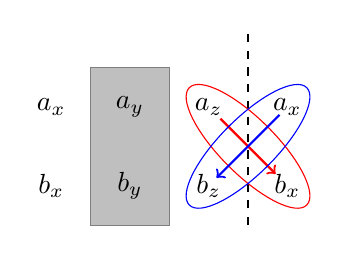
\begin{tikzpicture}[scale=1]

  \node at (0,1) {$a_x$};
  \node at (0,0) {$b_x$};

  \draw [fill=gray, opacity =0.5] (0.5, -0.5) rectangle (1.5,1.5) ;

  \node at (1,1) {$a_y$};
  \node at (1,0.0) {$b_y$};

  \node at (2,1) {$a_z$};
  \node at (2,0) {$b_z$};

  \draw [dashed] (2.5,-0.5) -- (2.5,2);

  \node at (3,1) {$a_x$};
  \node at (3,0) {$b_x$};

  \draw[rotate around={45:(2.5,0.5)},red] (2.5,0.5) ellipse (10pt and 30pt);

  \draw[->, red, thick] (2.15,0.85) -- (2.85,0.15);

  \draw[rotate around={-45:(2.5,0.5)},blue] (2.5,0.5) ellipse (10pt and 30pt);

  \draw[->, blue,thick] (2.90,0.90) -- (2.10,0.10);

\end{tikzpicture}
\end{document}
